\documentclass[../00_Main.tex]{subfiles}
\begin{document}

\subsection{La enfermedad.}
La esclerosis lateral amiotrófica o ELA, es una enfermedad degenerativa de las neuronas en el cerebro, el tronco cerebral y la médula espinal que controlan el movimiento de los músculos voluntarios. En la ELA, las células nerviosas (neuronas) motoras se desgastan o mueren y ya no pueden enviar mensajes a los músculos. Con el tiempo, esto lleva a debilitamiento muscular, espasmos e incapacidad para mover los brazos, las piernas y el cuerpo. La afección empeora lentamente. Cuando los músculos en la zona torácica dejan de trabajar, se vuelve difícil o imposible respirar.
En pacientes con ELA de etapas intermedias y avanzadas, es necesario el uso de dispositivos tecnológicos para la comunicación, como el P300 Speller.

\subsection{El P300 Speller y el oddball paradigm (paradigma del bicho raro).}
El P300 Speller es un dispositivo que conforma uno de las BCI (Brain Computer Interfaces) más usados en este tipo de aplicaciones. Su funcionamiento se acoge al paradigma del bicho raro: al usuario/paciente se le presenta una matriz de caracteres de 6 por 6 (ver figura) de manera intermitente, sucesiva y aleatoria. La tarea del usuario/paciente será enfocar su atención en los caracteres de una palabra prescrita por el investigador; es decir, un carácter a la vez. Cuando éstas contienen el carácter deseado (es decir, una fila particular y una columna determinada) se registra el potencial evocado P300 en el registro del EEC.

\begin{figure}[h]
    \centering
    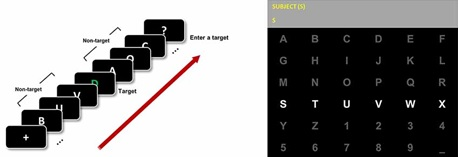
\includegraphics[[scale=1]{02_Images/Oddball}
    \caption{Paradigma del Oddball.}
    \label{fig:Oddball}
\end{figure}

\subsection{¿Qué es un ERP (Event Related Potential)?.}
De forma paralela, es necesario explicar qué es una señal P300. La palabra evocada es clave: en medicina, se refiere a una actividad que puede ser detectada sincrónicamente después de una cantidad específica de tiempo después del inicio de un estímulo. Si estamos a la espera de que un computador nos dé una señal visual y nos la da, en nuestro cerebro ocurre un evento de este tipo. En términos médicos es una \textit{actividad inducida}.

La onda P300 es entonces, una señal en el cerebro con amplitud positiva relacionada con eventos. Para esta investigación, los eventos serán aquellos provocados bajo \textit{el paradigma del bicho raro}: El sujeto detecta un estímulo "objetivo" ocasional en un tren regular de estímulos estándar. 

La onda P300 solo ocurre si el sujeto participa activamente en la tarea de detectar los objetivos. Su amplitud varía con la improbabilidad de los objetivos. Su latencia varía con la dificultad de discriminar el estímulo objetivo de los estímulos estándar. Una latencia pico típica cuando un sujeto adulto joven hace una discriminación simple es de 300 ms.

En pacientes con capacidad cognitiva disminuida, el P300 es más pequeño y más tardío que en sujetos normales de la misma edad.

\begin{figure}[H]
    \raggedright
    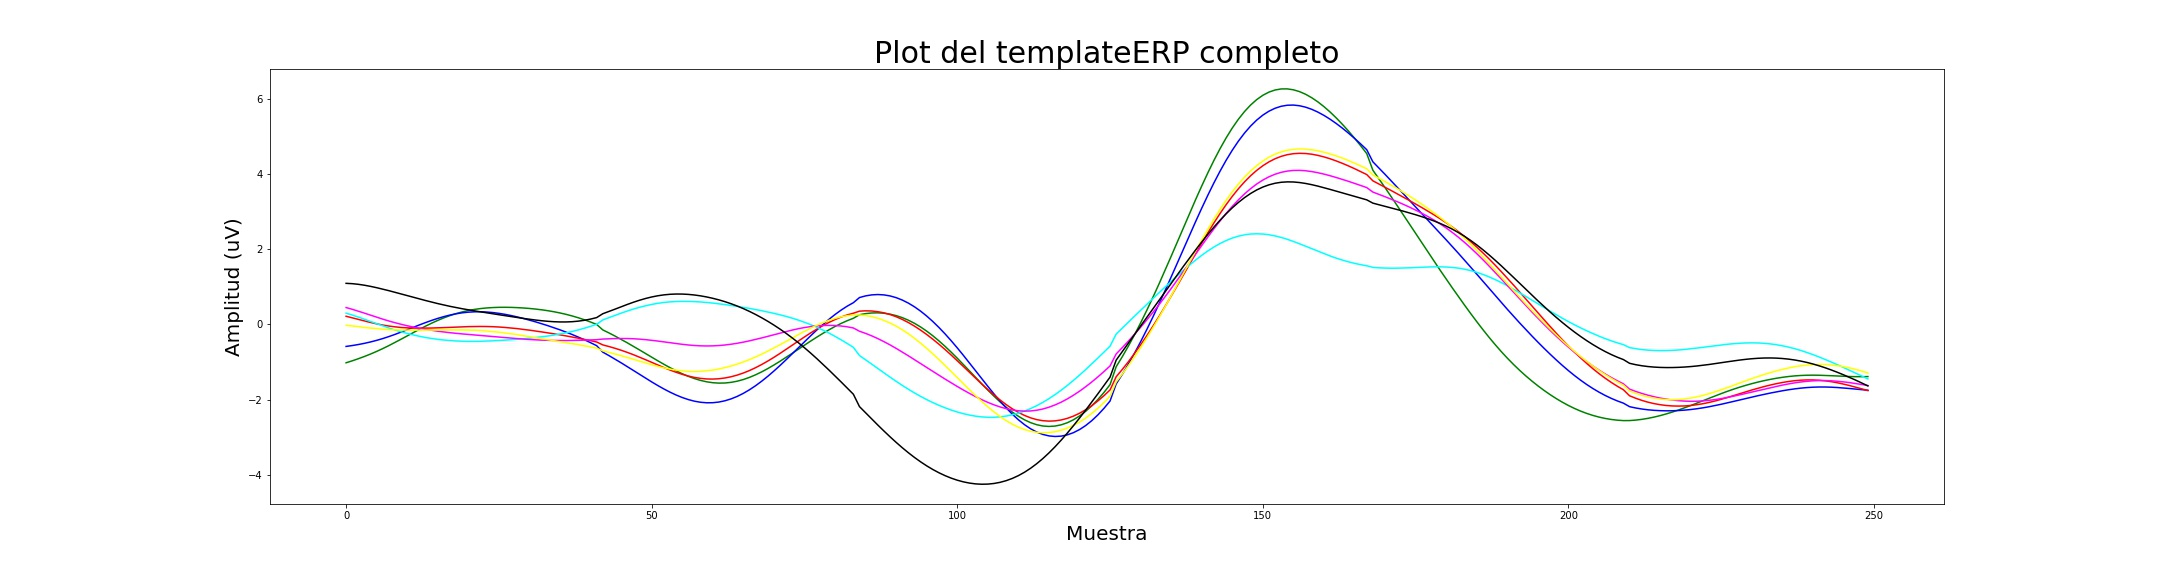
\includegraphics[scale=0.26]{02_Images/ERPTemplate}
    \caption{Señal: Event Related Potential.}
    \label{fig:ERPTemplate}
\end{figure}

El ERP P300 Puede tener una duración de 400ms y su amplitud puede alcanzar los 10µV (\cite{IntroductionBCIRao}). Se desconoce el origen intracerebral de la onda P300 y su papel en la cognición no se comprende con claridad. El P300 puede tener múltiples generadores intracerebrales, con el hipocampo y varias áreas de asociación de la neocorteza contribuyendo al potencial registrado en el cuero cabelludo. La onda P300 puede representar la transferencia de información a la conciencia, un proceso que involucra muchas regiones diferentes del cerebro (\cite{P300ofhumanERP}).

\subsection{Los datasets y las señales.}
Ya mencionado anteriormente, los electroencefalogramas que fueron usados son \textit{Matlab files}: archivos de extensión .mat en versiones con funcionalidades de almacenamiento de \textit{arrays} de n dimensiones de hasta 100.000.000 elementos por arreglo y 2^{31} bytes por variable. 

El dataset de \href{http://bnci-horizon-2020.eu/database/data-sets}{BNCI Horizon}, el 008-2014, contiene un grupo completo de potenciales evocados P300 registrados con la interfaz cerebro computador BCI2000 (\cite{schalk2004bci2000}). De éste dataset obtendremos el ERPTemplate. El otro, 

\href{https://www.kaggle.com/datasets/rramele/p300samplingdataset?resource=download}{el P300-Dataset}, está conformado por 8 EEGs de donde se extraerán algunos para realizar las pruebas del algoritmo. Todos los datasets están basados en el paradigma Farwell y Donchin (\cite{Talkinghead}) mencionado en el punto 9.2. Las señales usadas en este trabajo serán descritas a continuación:

\subsubsection{El ERPTemplate.}
Si bien la descripción de qué es un ERP está en el punto 9.3, es importante mencionar que éste ERP se extrae artificialmente del dataset de \href{http://bnci-horizon-2020.eu/database/data-sets}{BNCI Horizon} (008-2014) para ser “inyectado” a una señal EEG del \href{https://www.kaggle.com/datasets/rramele/p300samplingdataset?resource=download}{P300-Dataset} con el fin de crear una señal sintética que nos permita realizar las modificaciones de latencia y amplitud en donde quede empalmado dicho ERP.  El proceso está descrito en el punto 9.5. 

En \verb|a_analisis_ERPTemplate.ipynb| (\href{https://github.com/alexchavez1980/repo\_tesis}{repositorio de GitHub}) hay un análisis más en detalle de la estructura y propiedades de la onda.

%En el archivo *** hay un análisis más en detalle de la estructura y propiedades de la onda.

%\href{https://github.com/alexchavez1980/repo_tesis/blob/main/a_analisis_ERPTemplate.ipynb}{a_analisis_ERPTemplate.ipynb}

%\href{https://github.com/alexchavez1980/repo\_tesis}{En el repositorio de GitHub} podrás encontrar el archivo \textit{a_analisis_ERPTemplate.ipynb}

%\href{https://github.com/alexchavez1980/repo\_tesis}{En el repositorio de GitHub} podrás encontrar el archivo \verb|a_analisis_ERPTemplate.ipynb|

%\href{https://github.com/alexchavez1980/repo\_tesis}{\verb|a_analisis_ERPTemplate.ipynb|}

%\href{\url{https://github.com/alexchavez1980/repo\_tesis}
%{aanalisis_ERPTemplate.ipynb}}}

%\href{https://github.com/alexchavez1980/repo_tesis/blob/main/a_analisis_ERPTemplate.ipynb}{aanalisis_ERPTemplate.ipynb}

\subsubsection{P300-Dataset.}
El \href{https://www.kaggle.com/datasets/rramele/p300samplingdataset?resource=download}{P300-Dataset} está conformado por 8 EEGs distribuidos en dos grupos según la modalidad del experimento: pasivos P300S01,02,03,06 y activos P300S04, 05, 07 y 08. Este trabajo se enfoca en los pacientes pasivos: las trazas de EEG donde se superponen las pantillas ERP son de los pacientes que \textbf{no se enfocan en ninguna letra en particular}. Todo está allí, excepto el componente P300 ERP. Es por esto que se utiliza la información de marcadores para localizar los segmentos verdaderos donde se debería encontrar el P300, y esas ubicaciones de tiempo se utilizan para superponer la forma de onda de ERP extraída. 

\subsubsection{Estructura.}
El electroencefalograma obtenido se puede observar de dos maneras distintas: Una con cada una de sus componentes por separado, y la otra como una sola señal compuesta. Se utilizan en las ubicaciones Fz, Cz, Pz, Oz, P3, P4, PO7 y PO8 según el sistema internacional 10-20 para la colocación de los electrodos extracraneales. 

\begin{figure}[h]
    \centering
    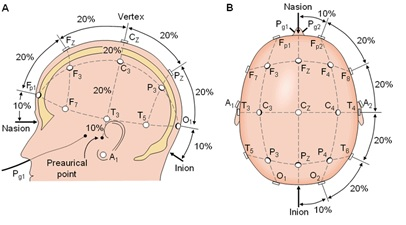
\includegraphics[[scale=1]{02_Images/posicion_electrodos02}
    \caption{Posicionamiento de los electrodos.}
    \label{fig:posicion_electrodos02}
\end{figure}

La referencia se establece en el lóbulo de la oreja derecha y la tierra está preestablecida como la posición AFz. La frecuencia de muestreo se establece en 250 Hz. \verb|a_analisis_P300XX.ipynb| (\href{https://github.com/alexchavez1980/repo\_tesis}{repositorio de GitHub}) es el análisis de dichas señales.

\begin{figure}[H]
    \raggedright
    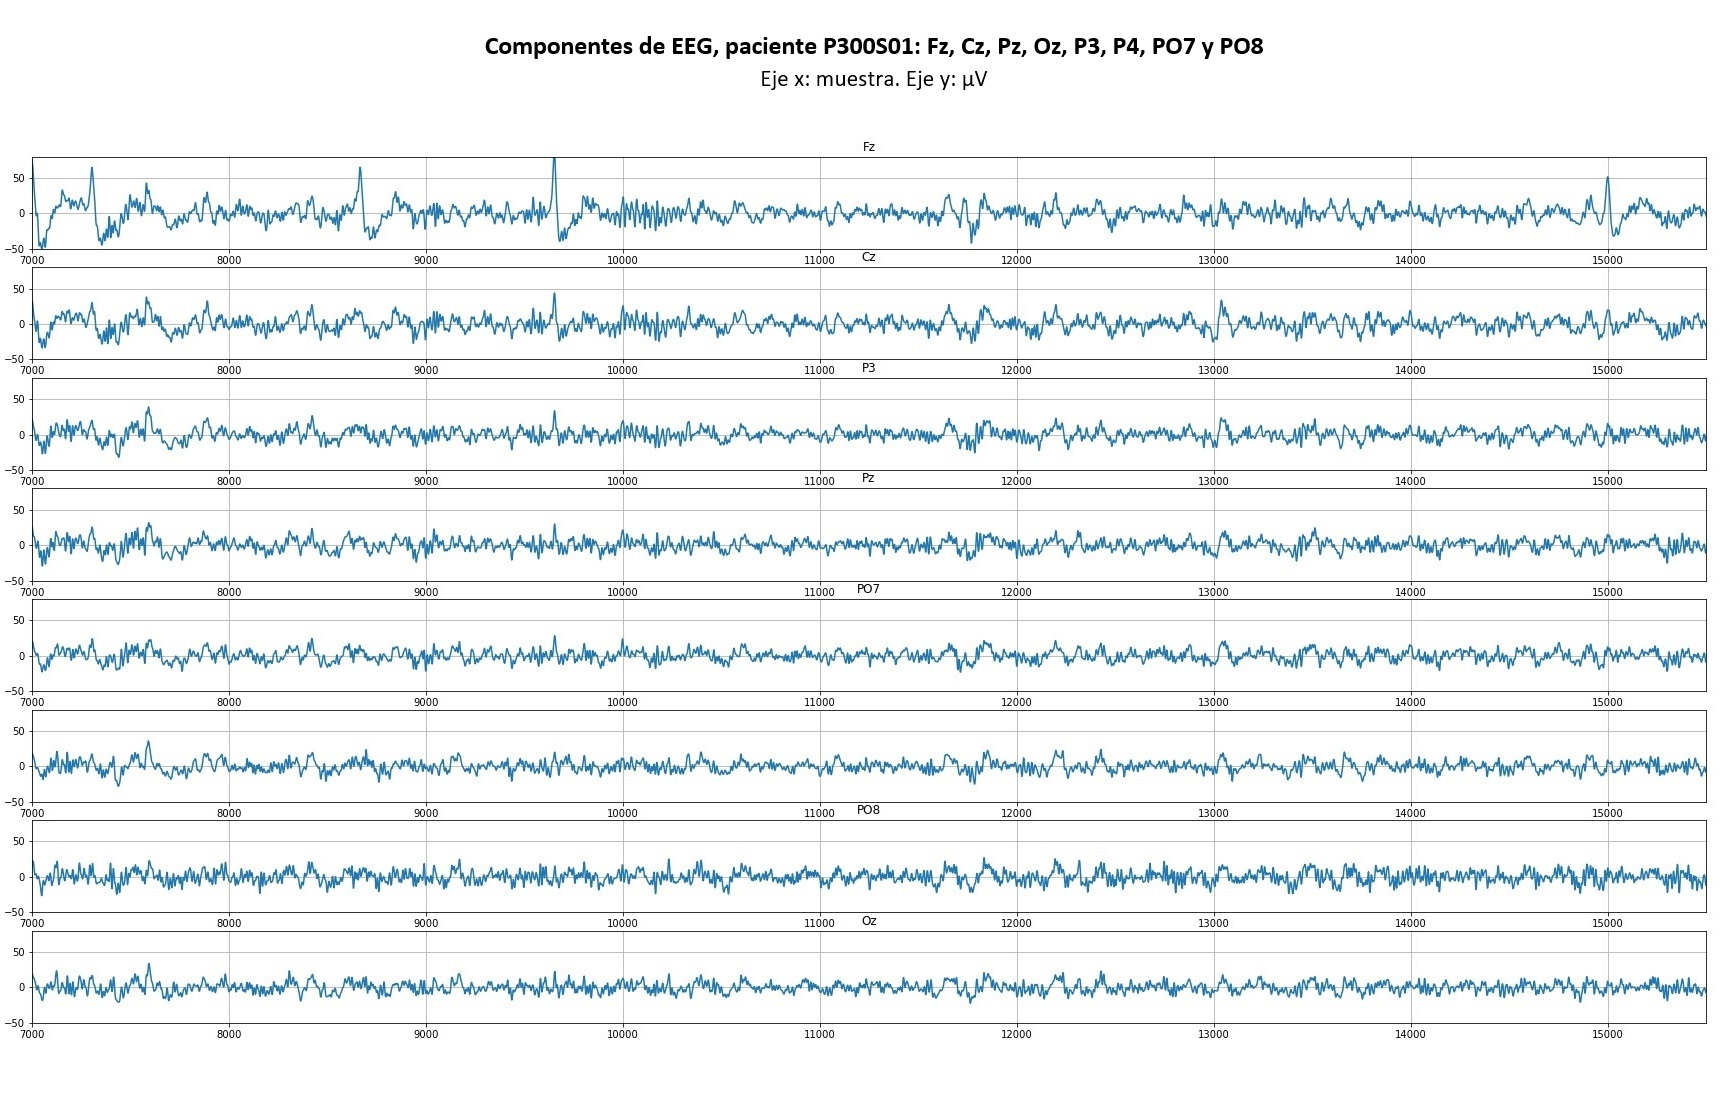
\includegraphics[scale=0.45]{02_Images/EEG}
    \caption{Detalle del electroencefalograma.}
    \label{fig:EEG}
\end{figure}

El archivo \textit{.mat} que contiene las señales obtenidas no solamente contiene las señales del electroencefalograma, sino las marcas del experimento. Es con ellas que se identifican dónde se encuentran los tiempos en donde se han mostrado los caracteres. 

\begin{figure}[H]
    \raggedright
    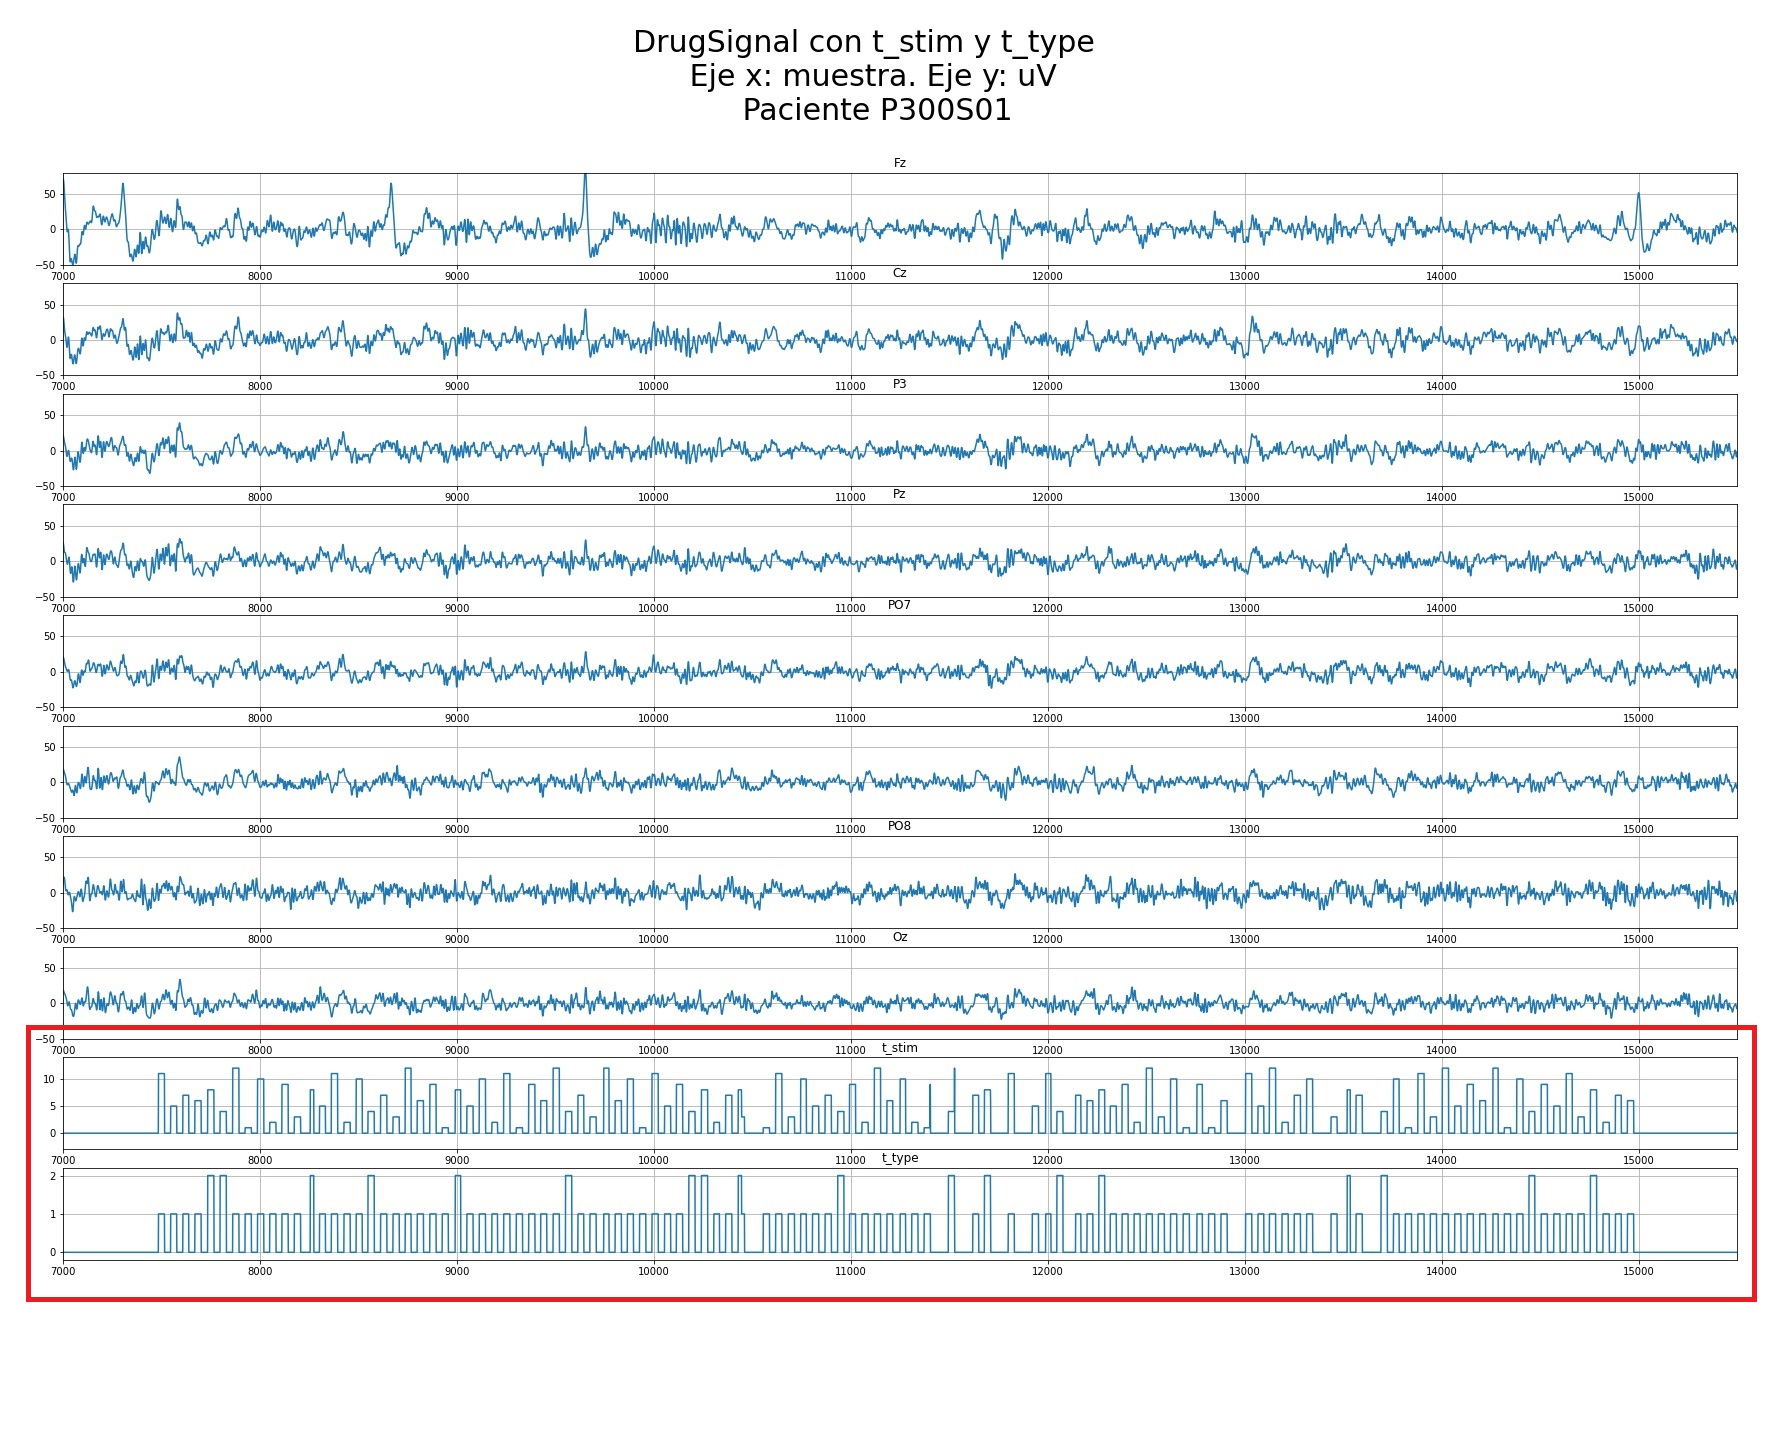
\includegraphics[scale=0.26]{02_Images/t_stim-t_type}
    \caption{Marcas del experimento.}
    \label{fig:t_stim-t_type}
\end{figure}

%\subsection{El ERPTemplate.}
%\large{\textbf{Alumno: Alexander Chavez Montaño}}\\

\biblio % Needed for referencing to working when compiling individual subfiles - Do not remove
\end{document}